\chapter{De Methodo Orationis Mentalis Francisci Salesi}
\begin{center}
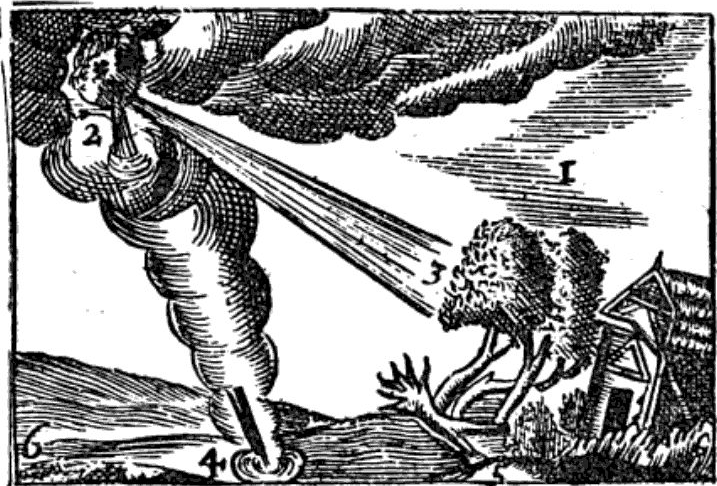
\includegraphics[scale=0.5]{Air.png}
\end{center}

\section{Intended Audience}
This is intended for students who have completed Lectio 7 and 8 of Latin by the Natural Method and Chapter 6 of Lingua Latina Per Se Illustrata. There are x words in this chapter.

Things to use:
	- Prope and Procul
	- Quam in comparison
	- Passive Verbs
	- Lots of Ablative
	- Locative Case 
	- Quo, Unde, Ubi
	- Fourth and Fifth Declension

\section{Text}
Silvae Jeremias et Eliseus ambulaverunt. Jeremias dixit ad Eliseum "Unde venisti?". "Natus sum Britanniae, Ubi sumus?". "Italiae sumus" Jeremias respondit. "Unde venisti?" interrogavit Eliseus. "Israel est ubi natus sum, ante Christum natum, sed natus es post Christum natum?". "Sum, duo milia anni post Christum natum.". Aura bona flat per arbores, et placet Jeremiae et Eliseo. "Bona aura est Silvae, flantur arbores.  Quo venit?" ait Eliseus. Respondit "Nescio. Deus scit, et scivit ante creationem mundi". "Sicut Deus spirat super nos.  Bene flat haec aura. Ignis non tam bonus est quam aura." ait Eliseus. "Quid? non placet tibi ignis meus? Aura tam bona non est quam ignis. Haec frigida aura non tam calida est quam ignis." respondit Jeremias. "Vetus vir!" exclamavit Eliseus "Senectus tuus cepit laetitiam bonae aurae ex te". "Cepit" respondit "Noli exclamare de hac re". "Sed" Jeremias addidit "non cepit Ventus Dei, flat in corde meo". 

"Quid est hic ventus?" interrogavit Eliseus. "Ventus, vel ignis orationis meae qui spirat in me". "Ignis? Quid ignis". "Ignis orationis mentalis" respondit "Qui instruxit me in amore et virtute, Ventus cognitionis Dei, non sicut scientia theologiae".  

\footnote{\textbf{ūrēbat} = It was burning}